\section{Memory Management}

\begin{frame}
  \frametitle{Physical and virtual memory}
  \begin{center}
    \includegraphics[height=0.8\textheight]{slides/kernel-driver-development-memory/mmu.pdf}
  \end{center}
\end{frame}

\begin{frame}
  \frametitle{Virtual memory organization}
  \begin{columns}
    \column{0.3\textwidth}
    \includegraphics[height=0.8\textheight]{slides/kernel-driver-development-memory/memory-organization.pdf}
    \column{0.7\textwidth}
    \begin{itemize}
    \item The top quarter reserved for kernel-space
      \begin{itemize}
      \item Contains kernel code and core data structures
      \item Allocations for loading modules
      \item All kernel physical mappings
      \item Identical in all address spaces
      \end{itemize}
    \item The lower part is a per user process exclusive mapping
      \begin{itemize}
      \item Process code and data (program, stack, ...)
      \item Memory-mapped files
      \item Each process has its own address space!
      \end{itemize}
    \item The exact virtual mapping in-use is displayed in the kernel log
      early at boot time
    \end{itemize}
  \end{columns}
\end{frame}

\begin{frame}
  \frametitle{Physical/virtual memory mapping on 32-bit systems}
  \begin{center}
    \includegraphics[height=0.8\textheight]{slides/kernel-driver-development-memory/memory-mapping-32b.pdf}
  \end{center}
\end{frame}

\begin{frame}
  \frametitle{32-bit systems limitations}
  \begin{itemize}
  \item Only less than 1GB memory addressable directly through kernel
    virtual addresses
  \item If more physical memory is present on the platform, part of
    the memory will not be accessible by kernel space, but can be used
    by user space
  \item To allow the kernel to access more physical memory:
    \begin{itemize}
    \item Change the 3GB/1GB memory split to 2GB/2GB or 1GB/3GB
      (\kconfig{CONFIG_VMSPLIT_2G} or \kconfig{CONFIG_VMSPLIT_1G)}
      $\Rightarrow$ reduce total user memory available for each process
    \item Activate \emph{highmem} support if available for your
      architecture:
      \begin{itemize}
      \item Allows kernel to map parts of its non-directly accessible
            memory
      \item Mapping must be requested explicitly
      \item Limited addresses ranges reserved for this usage
      \end{itemize}
    \end{itemize}
  \item See Arnd Bergmann's {\em 4GB by 4GB split} presentation
        (\href{https://resources.linaro.org/en/resource/TXkzgNDFp3HiJKdfQjbssL}
        {video and slides}) at Linaro Connect virtual 2020.
  \end{itemize}
\end{frame}

\begin{frame}
  \frametitle{Physical/virtual memory mapping on 64-bit systems (4kiB-pages)}
  \begin{center}
    \includegraphics[height=0.8\textheight]{slides/kernel-driver-development-memory/memory-mapping-64b.pdf}
  \end{center}
\end{frame}

\begin{frame}
  \frametitle{User space virtual address space}
  \begin{columns}
    \column{0.3\textwidth}
    \begin{itemize}
    \item When a process starts, the executable code is loaded in RAM and
      mapped into the process virtual address space.
    \item During execution, additional mappings can be created:
      \begin{itemize}
      \item Memory allocations
      \item Memory mapped files
      \item \code{mmap}'ed areas
      \item ...
      \end{itemize}
    \end{itemize}
    \column{0.7\textwidth}
    \includegraphics[height=0.7\textheight]{slides/kernel-driver-development-memory/userspace-mappings.pdf}
  \end{columns}
\end{frame}

\begin{frame}{Userspace memory allocations}
  \begin{itemize}
  \item Userspace mappings can target the full memory
  \item When allocated, memory may not be physically allocated:
    \begin{itemize}
    \item Kernel uses demand fault paging to allocate the physical
      page (the physical page is allocated when access to the virtual
      address generates a page fault)
    \item ... or may have been swapped out, which also induces a page
      fault
      \begin{itemize}
      \item See the \code{mlock}/\code{mlockall} system calls for
        workarounds
      \end{itemize}
    \end{itemize}
  \item User space memory allocation is allowed to over-commit memory
    (more than available physical memory) $\Rightarrow$ can lead to
    out of memory situations.
    \begin{itemize}
    \item Can be prevented with the use of
      \path{/proc/sys/vm/overcommit_*}
    \end{itemize}
  \item OOM killer kicks in and selects a process to kill to retrieve
    some memory. That's better than letting the system freeze.
  \end{itemize}
\end{frame}

\begin{frame}
  \frametitle{Kernel memory allocators}
  \begin{center}
    \includegraphics[height=0.8\textheight]{slides/kernel-driver-development-memory/allocators.pdf}
  \end{center}
\end{frame}

\begin{frame}[fragile]
  \frametitle{Page allocator}
  \begin{itemize}
  \item Appropriate for medium-size allocations
  \item A page is usually 4K, but can be made greater in some
    architectures (sh, mips: 4, 8, 16 or 64 KB, but not configurable in
    x86 or arm).
  \item Buddy allocator strategy, so only allocations of power of two
    number of pages are possible: 1 page, 2 pages, 4 pages, 8 pages,
    16 pages, etc.
  \item Typical maximum size is 8192 KB, but it might depend on the
    kernel configuration.
  \item The allocated area is contiguous in the kernel virtual address
    space, but also maps to physically contiguous pages. It is
    allocated in the identity-mapped part of the kernel memory space.
    \begin{itemize}
    \item This means that large areas may not be available or hard to
      retrieve due to physical memory fragmentation.
    \item The {\em Contiguous Memory Allocator} (\code{CMA}) can be used
      to reserve a given amount of memory at boot (see
      \url{https://lwn.net/Articles/486301/}).
    \end{itemize}
  \end{itemize}
\end{frame}

\begin{frame}[fragile]
  \frametitle{Page allocator API: get free pages}
  \begin{itemize}
  \item \mint{c}+unsigned long get_zeroed_page(gfp_t gfp_mask)+
    \begin{itemize}
    \item Returns the virtual address of a free page, initialized to
      zero
    \item \code{gfp_mask}: see the next pages for details.
    \end{itemize}
  \item \mint{c}+unsigned long __get_free_page(gfp_t gfp_mask)+
    \begin{itemize}
    \item Same, but doesn't initialize the contents
    \end{itemize}
  \item \mint{c}+unsigned long __get_free_pages(gfp_t gfp_mask, unsigned int order)+
    \begin{itemize}
    \item Returns the starting virtual address of an area of several
      contiguous pages in physical RAM, with order being
      \code{log2(number_of_pages)}.Can be computed
      from the size with the \kfunc{get_order} function.
    \end{itemize}
  \end{itemize}
\end{frame}

\begin{frame}[fragile]
  \frametitle{Page allocator API: free pages}
  \begin{itemize}
  \item \mint{c}+void free_page(unsigned long addr)+
    \begin{itemize}
    \item Frees one page.
    \end{itemize}
  \item \mint{c}+void free_pages(unsigned long addr, unsigned int order)+
    \begin{itemize}
    \item Frees multiple pages. Need to use the same order as in
      allocation.
    \end{itemize}
  \end{itemize}
\end{frame}

\begin{frame}
  \frametitle{Page allocator flags}
  The most common ones are:
  \begin{itemize}
  \item \ksym{GFP_KERNEL}
    \begin{itemize}
    \item Standard kernel memory allocation. The allocation may
      block in order to find enough available memory. Fine for most
      needs, except in interrupt handler context.
    \end{itemize}
  \item \ksym{GFP_ATOMIC}
    \begin{itemize}
    \item RAM allocated from code which is not allowed to block
      (interrupt handlers or critical sections). Never blocks,
      allows to access emergency pools, but can fail if no free
      memory is readily available.
    \end{itemize}
  \item Others are defined in \kfile{include/linux/gfp_types.h}.\\
      See also the documentation in \kdochtml{core-api/memory-allocation}
  \end{itemize}
\end{frame}

\begin{frame}
  \frametitle{SLAB allocator 1/2}
  \begin{itemize}
  \item The SLAB allocator allows to create {\em caches}, which contain a
    set of objects of the same size. In English, {\em slab} means {\em tile}.
  \item The object size can be smaller or greater than the page size
  \item The SLAB allocator takes care of growing or reducing the size
    of the cache as needed, depending on the number of allocated
    objects. It uses the page allocator to allocate and free pages.
  \item SLAB caches are used for data structures that are present in
    many instances in the kernel: directory entries, file
    objects, network packet descriptors, process descriptors, etc.
    \begin{itemize}
    \item See \code{/proc/slabinfo}
    \end{itemize}
  \item They are rarely used for individual drivers.
  \item See \kfile{include/linux/slab.h} for the API
\end{itemize}
\end{frame}

\begin{frame}
  \frametitle{SLAB allocator 2/2}
  \begin{center}
    \includegraphics[height=0.8\textheight]{slides/kernel-driver-development-memory/slab-allocator.pdf}
  \end{center}
\end{frame}

\begin{frame}[fragile]
  \frametitle{Different SLAB allocators}
  \small
  There are different, but API compatible, implementations of
  a SLAB allocator in the Linux kernel. A particular implementation
  is chosen at configuration time.
  \begin{itemize}
  \item \kconfig{CONFIG_SLAB}: legacy but now deprecated
  \item \kconfig{CONFIG_SLUB}: the default allocated, scaling better and creating less
        fragmentation than previous implementations.
  \item \kconfig{CONFIG_SLUB_TINY}: configure SLUB to achieve minimal memory
	footprint, sacrificing scalability, debugging and other
        features. Not recommended for systems with more than 16 MB of RAM.
  \end{itemize}
  \begin{center}
    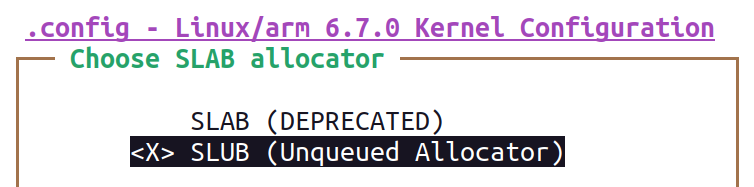
\includegraphics[height=0.2\textheight]{slides/kernel-driver-development-memory/slab-screenshot.png}
  \end{center}
\end{frame}

\begin{frame}
  \frametitle{kmalloc allocator}
  \begin{itemize}
  \item The kmalloc allocator is the general purpose memory allocator
    in the Linux kernel
  \item For small sizes, it relies on generic SLAB caches, named
    \code{kmalloc-XXX} in \code{/proc/slabinfo}
  \item For larger sizes, it relies on the page allocator
  \item The allocated area is guaranteed to be physically contiguous
  \item The allocated area size is rounded up to the size of the
        smallest SLAB cache in which it can fit
        (while using the SLAB allocator directly allows to have more
        flexibility)
  \item It uses the same flags as the page allocator (\ksym{GFP_KERNEL},
    \ksym{GFP_ATOMIC}, etc.) with the same semantics.
  \item Maximum sizes, on \code{x86} and \code{arm} (see
    \url{https://j.mp/YIGq6W}): \\
    - Per allocation: 4 MB \\
    - Total allocations: 128 MB
  \item Should be used as the primary allocator unless there is a
    strong reason to use another one.
  \end{itemize}
\end{frame}

\begin{frame}[fragile]
  \frametitle{kmalloc API 1/2}
  \begin{itemize}
  \item \mint{c}+#include <linux/slab.h>+
  \item \mint{c}+void *kmalloc(size_t size, gfp_t flags);+
    \begin{itemize}
    \item Allocate \code{size} bytes, and return a pointer to the area
      (virtual address)
    \item \code{size}: number of bytes to allocate
    \item \code{flags}: same flags as the page allocator
    \end{itemize}
  \item \mint{c}+void kfree(const void *objp);+
    \begin{itemize}
    \item Free an allocated area
    \end{itemize}
  \item Example: (\kfile{drivers/infiniband/core/cache.c})
\begin{minted}{c}
struct ib_port_attr *tprops;
tprops = kmalloc(sizeof *tprops, GFP_KERNEL);
...
kfree(tprops);
\end{minted}
  \end{itemize}
\end{frame}

\begin{frame}[fragile]
  \frametitle{kmalloc API 2/2}
  \begin{itemize}
  \item \mint{c}+void *kzalloc(size_t size, gfp_t flags);+
    \begin{itemize}
    \item Allocates a zero-initialized buffer
    \end{itemize}
  \item \mint{c}+void *kcalloc(size_t n, size_t size, gfp_t flags);+
    \begin{itemize}
    \item Allocates memory for an array of \code{n} elements of
      \code{size} size, and zeroes its contents.
    \end{itemize}
  \item \mint{c}+void *krealloc(const void *p, size_t new_size, gfp_t flags);+
    \begin{itemize}
    \item Changes the size of the buffer pointed by \code{p} to
      \code{new_size}, by reallocating a new buffer and copying the
      data, unless \code{new_size} fits within the alignment of
      the existing buffer.
    \end{itemize}
  \end{itemize}
\end{frame}

\begin{frame}
  \frametitle{devm\_kmalloc functions}
  Allocations with automatic freeing when the corresponding device or module is unprobed.
  \begin{itemize}
  \small
  \item \mint{c}+void *devm_kmalloc(struct device *dev, size_t size, gfp_t gfp);+
  \item \mint{c}+void *devm_kzalloc(struct device *dev, size_t size, gfp_t gfp);+
  \item \mint{c}+void *devm_kcalloc(struct device *dev, size_t n, size_t size, gfp_t flags);+
  \item \mint{c}+void *devm_kfree(struct device *dev, void *p);+
        Useful to immediately free an allocated buffer
  \end{itemize}
  \normalsize
  For use in \code{probe()} functions, in which you have access to a
  \kstruct{device} structure.
\end{frame}

\begin{frame}[fragile]
  \frametitle{vmalloc allocator}
  \begin{itemize}
  \item The \kfunc{vmalloc} allocator can be used to obtain
    memory zones that are contiguous in the virtual addressing space,
    but not made out of physically contiguous pages.
  \item The requested memory size is rounded up to the next page (not
    efficient for small allocations).
  \item The allocated area is in the kernel space part of the address
    space, but outside of the identically-mapped area
  \item Allocations of fairly large areas is possible (almost as big
    as total available memory, see \url{https://j.mp/YIGq6W} again),
    since physical memory fragmentation is not an issue.
  \item Not suitable for DMA purposes.
  \item API in \kfile{include/linux/vmalloc.h}
    \begin{itemize}
    \item \mint{c}+void *vmalloc(unsigned long size);+
      \begin{itemize}
      \item Returns a virtual address
      \end{itemize}
    \item \mint{c}+void vfree(void *addr);+
    \end{itemize}
  \end{itemize}
\end{frame}

\begin{frame}
  \frametitle{Kernel memory debugging}
  \begin{itemize}
  \item \code{KASAN} ({\em Kernel Address Sanitizer})
    \begin{itemize}
    \item Dynamic memory error detector, to find use-after-free and
      out-of-bounds bugs.
    \item Available on most architectures
    \item See \kdochtml{dev-tools/kasan} for details.
    \end{itemize}
  \item \code{KFENCE} ({\em Kernel Electric Fence})
    \begin{itemize}
    \item A low overhead alternative to KASAN, trading performance
	  for precision. Meant to be used in production systems.
    \item Available on most architectures.
    \item See \kdochtml{dev-tools/kfence} for details.
    \end{itemize}
  \item \code{Kmemleak}
    \begin{itemize}
    \item Dynamic checker for memory leaks
    \item This feature is available for all architectures.
    \item See \kdochtml{dev-tools/kmemleak} for details.
    \end{itemize}
  \end{itemize}
  KASAN and Kmemleak have a significant overhead. Only use them in development!
\end{frame}

\begin{frame}
  \frametitle{Kernel memory management: resources}
  Virtual memory and Linux, Alan Ott and Matt Porter, 2016\\
  Great and much more complete presentation about this topic\\
  \url{https://bit.ly/2Af1G2i} (video: \url{https://bit.ly/2Bwwv0C})
  \begin{center}
     \includegraphics[height=0.6\textheight]{slides/kernel-driver-development-memory/ott-porter-kernel-virtual-memory-presentation.jpg}
  \end{center}
\end{frame}
